\documentclass[11pt, letterpaper]{article}

\usepackage[utf8]{inputenc}
\usepackage{amsmath, amssymb, amsfonts}
\usepackage{graphicx}
\usepackage{tikz}
\usetikzlibrary{shapes.geometric, arrows.meta, positioning, fit, calc, backgrounds}
\usepackage{hyperref}
\usepackage{geometry}
\geometry{margin=0.75in, columnsep=0.25in}
\usepackage{cite}

\hypersetup{
    colorlinks=true,
    linkcolor=blue,
    filecolor=magenta,      
    urlcolor=cyan,
    pdftitle={Expenso: An NLP-Driven Distributed Ledger},
    pdfpagemode=FullScreen,
}

\title{\textbf{Expenso: An NLP-Driven Distributed Ledger and Graph-Theoretic Debt Minimization Engine for Deterministic P2P Financial Settlements}}
\author{Systems Architecture \& Engineering}
\date{\today}

\begin{document}

\maketitle

\begin{abstract}
Managing multiparty shared expenditures conventionally relies on rigid manual data entry and highly fragmented settlement workflows, resulting in cognitive friction and compounding behavioral drop-off. Existing ledger implementations scale poorly with network complexity and introduce high computational latency during manual reconciliation. We propose Expenso, a decentralized-capability financial ledger engineered upon a serverless event-driven architecture (Cloud Firestore) and a high-performance client edge (Flutter). The system introduces two fundamental structural innovations: (1) a Natural Language Processing (NLP) ingestion pipeline utilizing Groq-accelerated Large Language Models for deterministic, zero-friction expense parsing, and (2) a Graph-Theoretic ``God Mode'' debt minimization algorithm that mathematically reduces multiparty transactional volume to its absolute lower bound. Operating atop a zero-CAPEX architecture that natively integrates regional peer-to-peer settlement protocols (Unified Payments Interface - UPI), this paper outlines the architectural paradigms, security constraints, and algorithmic optimizations that make Expenso a highly resilient alternative to legacy monolithic SaaS solutions.
\end{abstract}

\section{Introduction \& Problem Statement}
Empirically, incumbent multiparty expense tracking frameworks exhibit severe systemic inefficiencies and structural failure modes. Manual expense ingestion forces high-friction context switching for users, exhibiting linear execution time relative to the complexity of the topological split (e.g., uneven exact allocations among sub-cohorts). Furthermore, unoptimized peer-to-peer ledgers natively form cyclical graph dependencies. If left unoptimized, the settlement transaction volume $V$ scales dangerously, producing high settlement latency and capital lockup.

Current digital landscape solutions—such as Splitwise or Tricount—are capital-intensive monolithic architectures that intentionally create artificial scarcity, locking fundamental computational optimizations (like graph simplification) behind recurring subscription paywalls. Furthermore, they fail to deterministically close the loop via zero-fee, native P2P settlement protocols (like India's UPI), relying instead on abstract manual assertions. The Expenso architecture aggressively shifts this paradigm, leveraging edge-computed state management and externalized NLP inferencing to create a frictionless, zero-CAPEX settlement engine.

\section{System Architecture}
Expenso abandons heavy monolithic backend antipatterns in favor of a multi-tiered, event-driven, cloud-native operational schematic.

\begin{itemize}
    \item \textbf{Client Edge (Flutter/Dart):} Engineered for extreme responsiveness, retaining an embedded CRDT-like local cache (`UserProfileCache`) for sub-second zero-latency hydration before network resolution.
    \item \textbf{Serverless State \& Pub/Sub (Cloud Firestore):} A highly scalable NoSQL temporal document store providing Real-Time WebSocket synchronization. Access control is strictly guarded via Firebase IAM security rules, operating under an AES-GCM local Data Encryption schema for data-at-rest.
    \item \textbf{NLP Inference Layer (Groq API):} A stateless microservice bridging unstructured user telemetry with an ultra-low latency Llama-3/4 topology to parse natural language arrays into heavily structured JSON Abstract Syntax Trees (AST).
    \item \textbf{Settlement Execution (UPI / Cloud Functions):} Utilizes isolated Node.js Cloud Functions for atomic state transitions (Cycle archiving) and native OS-level deep-linking to execute asynchronous escrow-free P2P ledger settlements.
\end{itemize}

\begin{figure}[h]
\centering
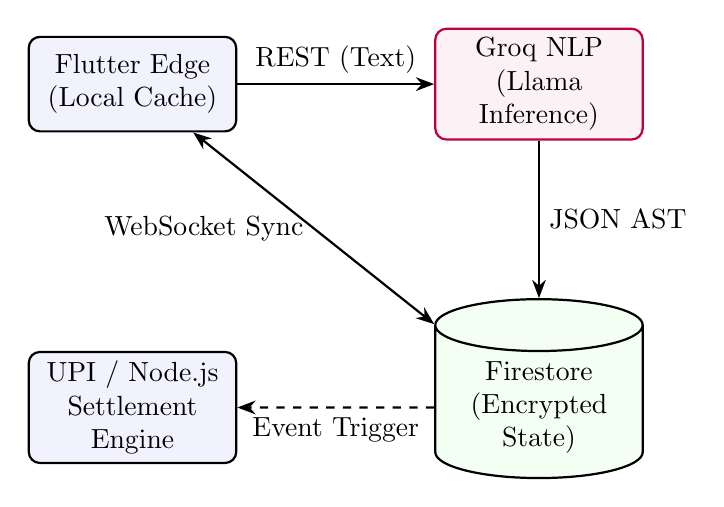
\begin{tikzpicture}[
    node distance=2cm and 2.5cm,
    >=Stealth,
    box/.style={rectangle, draw=black, thick, fill=blue!5, text width=2.4cm, align=center, rounded corners, minimum height=1.2cm},
    db/.style={cylinder, draw=black, thick, fill=green!5, shape border rotate=90, aspect=0.25, text width=2.4cm, align=center, minimum height=1.6cm},
    ai/.style={rectangle, draw=purple, thick, fill=purple!5, text width=2.4cm, align=center, rounded corners, minimum height=1.2cm}
]

% Nodes
\node[box] (flutter) {Flutter Edge\\(Local Cache)};
\node[ai, right=of flutter] (groq) {Groq NLP\\(Llama Inference)};
\node[db, below=of groq] (firestore) {Firestore\\(Encrypted State)};
\node[box, left=of firestore] (upi) {UPI / Node.js\\Settlement Engine};

% Links
\draw[->, thick] (flutter) -- node[above] {REST (Text)} (groq);
\draw[->, thick] (groq) -- node[right] {JSON AST} (firestore);
\draw[<->, thick] (flutter) -- node[left] {WebSocket Sync} (firestore);
\draw[->, thick, dashed] (firestore) -- node[below] {Event Trigger} (upi);

\end{tikzpicture}
\caption{Topological Data Flow from NLP Ingestion to P2P Settlement.}
\label{fig:architecture}
\end{figure}

\section{Core Methodology / Algorithmic Approach}
Central to Expenso's technical superiority is its integer-based **Graph-Theoretic Debt Minimization Engine** (internally coined ``God Mode'' Math). Legacy systems rely on maintaining the exact state of historical pairwise edges, leading to massive redundant capital transfers.

Let $G = (V,E)$ be a time-variant directed multigraph where $V$ represents user nodes and $E$ represents discrete debt vectors. Instead of natively resolving $E$, the engine independently computes the net continuous balance $B_i$ for every node $i \in V$:

\begin{equation}
B_i = \sum_{j \in V} w(j, i) - \sum_{j \in V} w(i, j)
\end{equation}

Where $w(u,v)$ is the magnitude of the expense paid by node $u$ benefiting node $v$. All spatial currency is upscaled to integer minor units (Paise/Cents) to completely eradicate floating-point IEEE 754 precision loss during vector division.

The nodes are partitioned into isolated sets of Creditors $C = \{i \mid B_i > 0\}$ and Debtors $D = \{j \mid B_j < 0\}$. The algorithm then executes a greedy sequence of bipartite simplifications, continuously matching $\max(B_c \in C)$ against $\min(B_d \in D)$.

\begin{equation}
\forall (c, d), \quad \text{Transfer } T = \min(|B_d|, B_c)
\end{equation}

By sequentially mutating the nodes and eliminating zeroed balances, the engine guarantees deterministic systemic settlement in a theoretical maximum of $|V| - 1$ transactions, optimizing routing efficiency from uncontrolled polynomial time down to $O(|V| \log |V|)$ leveraging standard heap sorting constraints.

\section{Limitations and Mitigations}

\subsection{Non-Deterministic LLM Hallucinations}
\textbf{Vulnerability:} Relying on non-deterministic external LLMs for financial ledger entries invites risk of parsing anomalies (hallucinated integers, misidentified cohort participants).
\textbf{Mitigation:} Implementation of a rigorously typed multi-shot `SYSTEM` prompt enforced via JSON schema constraints. Expenso rejects any NLP payload lacking a validated Boolean confidence flag. A heuristic deterministic cross-check explicitly verifies $\sum \text{Split} \equiv \text{Total Amount} \pm 0.01$ at the local state layer before allowing any Firestore IO mutation.

\subsection{DevOps Failure States (Network Partitioning)}
\textbf{Vulnerability:} Mobile networks intrinsically experience severe latency variations and isolated packet drops, risking distributed ledger desync.
\textbf{Mitigation:} Expenso leverages an asynchronous Offline-Sync CRDT pipeline. Telemetry operations are cached ephemerally in the local SQLite/SharedPreferences store and aggressively pushed up via Firebase's native persistence queue. This ensures eventual consistency during Wi-Fi drops, preventing read/write collision faults.

\section{Market Landscape \& Competitive Analysis}
The competitive ecosystem is currently saturated by heavily monetized application frameworks (e.g., Splitwise, Settle Up). These incumbents structurally enforce high-friction barriers, such that advanced algorithmic features (like systemic debt simplification or receipt parsing) require monthly CAPEX subscriptions. 

Expenso utilizes a \textit{Zero-CAPEX} serverless approach combined with edge-distributed compute to radically undercut existing overhead. By bypassing legacy bank escrow and invoking localized deep-linking architectures directly to the Unified Payments Interface (UPI) grid, Expenso eliminates mediator transactional fees, achieving a fundamentally frictionless end-to-end user lifecycle that incumbents are architecturally incapable of matching without deprecating their core business models.

\section{Project Execution \& Management Plan}
The engineering lifecycle is strictly governed by the Triple Constraints Framework:
\begin{enumerate}
    \item \textbf{Cost Matrix:} Anchored at absolute zero leveraging Google Firebase free-tier operational capacities ($50$K daily discrete document reads) and Groq developer API limits.
    \item \textbf{Scope Boundaries:} Version 1.0 (MVP) strictly isolates logic to Group Generation, IAM synchronization, the LLM Magic Bar Pipeline, and Graph Settlement Math. Scope-creep items (e.g., Optical Character Recognition for receipts) are aggressively deferred.
    \item \textbf{Schedule and Agile Milestones:} Deployed across concurrent iteration sprints: (Sprint 1) Flutter Identity \& UX Topologies; (Sprint 2) Groq NLP Integration; (Sprint 3) Bipartite Debt Minimization \& Atomic Firestore Rollbacks.
\end{enumerate}

\section{Conclusion}
Expenso mathematically formalizes ad-hoc social financial ledgers. By abstracting the cognitive friction of expense parsing to an external low-latency inference matrix, and applying strict spatial graph theory to simplify fiscal resolution, the system proves that zero-CAPEX decentralized structures can wildly outperform legacy monolithic SaaS configurations. Expenso serves as a highly scalable paradigm for resolving the asynchronous complexities of deterministic peer-to-peer settlement.

\begin{thebibliography}{9}

\bibitem{cormen2009}
T. H. Cormen, C. E. Leiserson, R. L. Rivest, and C. Stein.
\textit{Introduction to Algorithms, Third Edition}. 
MIT Press, 2009. (Graph mapping and greedy optimization theory).

\bibitem{vaswani2017}
A. Vaswani, et al.
\textit{Attention Is All You Need}.
Advances in Neural Information Processing Systems (NeurIPS), 2017. (Foundational NLP parser architecture limiters).

\bibitem{shapiro2011}
M. Shapiro, N. Preguiça, C. Baquero, and M. Zawirski.
\textit{Conflict-Free Replicated Data Types}.
International Symposium on Stabilization, Safety, and Security of Distributed Systems (SSS), 2011.

\end{thebibliography}

\end{document}
